% AAAI-27 submission — AI for Social Impact track
% aaai2027.sty / aaai2027.bst are vendored from the AAAI-27 author kit.
\documentclass[letterpaper]{article} % DO NOT CHANGE THIS
\usepackage[submission]{aaai2027}  % DO NOT CHANGE THIS
% Fonts (newtxtext, helvet, courier) are loaded by aaai2027.sty; do NOT add
% times/helvet/courier here — the style forbids it.
\usepackage[hyphens]{url}  % DO NOT CHANGE THIS
\usepackage{graphicx} % DO NOT CHANGE THIS
\urlstyle{rm} % DO NOT CHANGE THIS
\def\UrlFont{\rm}  % DO NOT CHANGE THIS
\usepackage{natbib}  % DO NOT CHANGE THIS AND DO NOT ADD ANY OPTIONS TO IT
\usepackage{caption} % DO NOT CHANGE THIS AND DO NOT ADD ANY OPTIONS TO IT
\frenchspacing  % DO NOT CHANGE THIS
\setlength{\pdfpagewidth}{8.5in}  % DO NOT CHANGE THIS
\setlength{\pdfpageheight}{11in}  % DO NOT CHANGE THIS
\usepackage{amsmath}
\usepackage{amssymb}
\usepackage{booktabs}

\pdfinfo{
/TemplateVersion (2027.1)
}

% Sections are referenced by number (\ref{sec:...}); enable numbering.
\setcounter{secnumdepth}{2}

\title{Listening Without Labels: Open-Set Acoustic Threat Detection\\
for Forest Conservation from Background Audio Alone}

% ---------------------------------------------------------------------------
% AUTHORSHIP.
% AAAI-27 main-track review is DOUBLE-BLIND: the submitted PDF must carry
% "Anonymous submission" only. The real author block below is for the
% camera-ready version. Do NOT uncomment it before acceptance -- naming
% authors in the submission de-anonymizes the paper and risks desk rejection.
%
% CAMERA-READY RESTORE: the platform name ("Canopy") is withheld throughout for
% anonymous review, since the public repository would identify the authors.
% Restore it in main.tex (abstract), sections/introduction.tex (contributions),
% and sections/deployment.tex (opening line) at camera-ready.
%
% NOTE: the [submission] option above hard-forces "Anonymous submission" in
% \maketitle (aaai2027.sty clears \showauthors@on), so uncommenting the block
% below is NOT enough on its own -- the option must also be dropped. A ready
% camera-ready driver that does both lives in main_cameraready.tex.
%
% Camera-ready block (add emails, then swap in for the two active lines below):
% \author{
%     Arjun Tyagi\textsuperscript{\rm 1}\thanks{Corresponding author.},
%     Arun Hariharan\textsuperscript{\rm 2},
%     Hriday Matharu\textsuperscript{\rm 1},
%     Pranav Tawakley\textsuperscript{\rm 3},
%     Tanush Jhamb\textsuperscript{\rm 4},
%     Tashi Shrivastava\textsuperscript{\rm 5}
% }
% \affiliations{
%     \textsuperscript{\rm 1}Pennsylvania State University\\
%     \textsuperscript{\rm 2}PES University, Bangalore\\
%     \textsuperscript{\rm 3}Manipal University\\
%     \textsuperscript{\rm 4}University of Essex\\
%     \textsuperscript{\rm 5}Somaiya Vidyavihar\\
%     % TODO before camera-ready: add contact email(s) and each author's
%     % department.
% }
% ---------------------------------------------------------------------------
\author{Anonymous submission}
\affiliations{Anonymous submission}

\begin{document}

\maketitle

\begin{abstract}
Acoustic monitoring is a scalable defense against illegal logging, but standard detectors, closed-set classifiers trained on public audio, fail on new forest sites. Using an audited, leakage-free, leave-one-site-out protocol across four rainforest locations, we show the breakdown is not in discrimination but in operating-point transfer: a classifier at $0.907$ in-domain accuracy detects essentially no chainsaws on any held-out site, even where its own score still ranks chainsaws above background at ROC-AUC $0.964$. A linear probe recovers recording site from the learned representation at $4\times$ chance and more strongly than it recovers event class, giving a mechanism for the failure. We propose a background-first, open-set detector that sidesteps the trap: it fits a density over a frozen general-purpose embedding on unlabeled deployment-site background, calibrates a threshold to an explicit background false-positive budget, and attributes flagged events with per-class prototypes built incrementally from ranger-verified positives, reserving honest \emph{unknown} mass otherwise. On the primary held-out site it reaches AUC $0.713$ and flags $0.317$ of chainsaws at a $0.056$ false-positive rate, exceeding the calibrated closed-set recall of $0.195$ while using zero labeled positives to decide what is anomalous. A supervised probe on the same frozen embeddings prices what label-free operation costs and isolates the binding constraint as representational: weighted AUROC is $0.783$ for AudioSet and $0.786$ for a bird-specific encoder (BirdNET), but only $0.648$ for the site-trained representation. Deployed in an open-source monitoring platform we release, ranger feedback closes the loop, with each verified alert becoming a prototype update and no retraining. We release code, fitted models, and the full protocol.
\end{abstract}

\section{Introduction}

Illegal logging is a leading driver of tropical forest loss, and its most
reliable early signature is sound: chainsaws, vehicles, and gunshots carry for
hundreds of meters under canopy that hides them from satellites for days to
weeks. Low-cost acoustic sensors are therefore among the most widely deployed
conservation technologies. The dominant recipe is a closed-set
classifier --- train a CNN on labeled clips of $k$ threat classes, deploy, and
alert when a class probability crosses a threshold.

This recipe embeds two assumptions that fail in conservation deployments.
First, it assumes labeled positives from the deployment domain exist. They
rarely do: a new reserve has no verified recordings of chainsaws \emph{under its
own microphones, weather, and species chorus}, and public datasets are dominated
by close-range, high-SNR urban recordings. Second, it assumes the threat
taxonomy is known in advance, so any sound outside the $k$ classes is silently
mapped onto them or suppressed.

We first quantify how badly the closed-set recipe travels. A CNN chainsaw
detector trained on rainforest soundscapes from multiple sites, with
leakage-checked splits and validation-calibrated thresholds, reaches only
$0.195$ recall on a fully held-out site at a deployable background
false-positive rate --- despite $0.976$ raw-argmax recall that would flag half
of all background as threats (Section~\ref{sec:experiments}). The model learns
a real chainsaw signal but not a decision boundary that transfers across sites. Our open-set detector, over a
frozen general-purpose audio embedding, recovers a deployable operating point on
the same held-out site --- $0.317$ flagged recall at $0.056$ background FP,
exceeding the closed-set calibrated recall while using no labeled positives to
decide what is anomalous.

We argue the deployable formulation is open-set and background-first:
\begin{enumerate}
\item \textbf{Flag} a clip by how far it deviates from \emph{this forest's}
      normal soundscape --- a density fit on unlabeled background audio alone,
      which every deployment can record on day one;
\item \textbf{Attribute} flagged clips against per-class prototypes built from
      whatever ranger-verified positives exist so far --- zero at launch;
\item \textbf{Abstain honestly}: when no prototype matches, report
      \emph{unknown} rather than forcing a known label.
\end{enumerate}
The decision threshold is calibrated to an explicit background false-positive
budget, because ranger attention --- not accuracy --- is the scarce resource.

Our contributions:
\begin{itemize}
\item A negative result with an audited protocol: closed-set acoustic threat
      classifiers do not learn deployable cross-site decision boundaries, even
      with in-domain multi-site training data.
\item A background-only open-set detector --- shrunk-covariance Mahalanobis
      density over a frozen pretrained embedding, quantile-mapped scores, an
      FP-budget threshold, and prototype attribution with reserved unknown
      mass --- that ships with zero labeled threats and improves monotonically
      as verified positives arrive, without retraining.
\item A site-held-out evaluation across RFCx rainforest sites measuring
      flagging, attribution, the attribution-vs-verified-positives curve, and
      honest-unknown behavior under class holdout. The embedding, not the
      detector head, is what governs cross-site deployability: a frozen AudioSet
      encoder clears chance-level separability at every site where the
      forest-CNN embedding does not.
\item An open-source deployment (Canopy) in which the ranger review loop
      closes the label flywheel: confirmed alerts become prototype updates.
\end{itemize}

\section{Related Work}
\label{sec:related}

\paragraph{Acoustic monitoring for conservation.} Passive acoustic monitoring is
established for biodiversity and increasingly for threat detection (chainsaws,
gunshots, vehicles), with deployments such as Rainforest Connection converting
recordings into ranger alerts \citep{stowell2022bioacoustics}. These systems
predominantly use closed-set supervised classifiers and report in-domain metrics; cross-site generalization
under a fixed false-positive budget is rarely measured. A global expert assessment of
PAM practice identifies manual validation of detector output as a priority
bottleneck \citep{malerba2026pam}, which is why we treat reviewer attention,
not accuracy, as the operative constraint. Our negative
result quantifies the cross-site gap this reflects, and our detector targets the
label-scarce, open-taxonomy regime deployments actually face.


\paragraph{Few-shot bioacoustic event detection.} The DCASE few-shot bioacoustic
task formalizes detecting novel sound events from a handful of labeled examples
\citep{nolasco2023dcase}. Our prototype stage is in this spirit, since a class is defined by a few
verified positives, but we couple it to a background-only anomaly gate and an
explicit unknown option, so the system flags before any labels exist and
abstains when no prototype matches.


\paragraph{Open-set recognition and OOD detection.} Open-set recognition asks a
classifier to reject inputs outside its training classes; a large OOD-detection
literature scores novelty, including Mahalanobis distance in a deep feature
space \citep{lee2018mahalanobis}. We adopt the Mahalanobis-in-embedding scoring but invert the usual
framing: the ``in-distribution'' density is \emph{normal forest background}, not
the labeled classes, so the detector is trained without any positives and known
classes enter only as post-hoc prototypes.


\paragraph{Prototypical and metric learning.} Class-mean prototypes with cosine
similarity are standard in few-shot metric learning \citep{snell2017prototypical}. Our contribution is not the
prototype but its role in a deployable pipeline: prototypes are optional,
incrementally updatable from human confirmations, and gated behind a
background-calibrated anomaly threshold with reserved unknown mass.


\paragraph{Transfer of pretrained audio embeddings.} Large audio taggers pretrained on AudioSet \citep{gemmeke2017audioset}, such as
CNN14 \citep{kong2020panns}, yield general-purpose embeddings that transfer
across audio tasks, as does the bioacoustics-specific BirdNET
\citep{kahl2021birdnet}. We use one as a frozen $\phi$ and show that the choice of embedding,
not the detector head, governs cross-site deployability for forest threats.


\paragraph{Distribution shift, shortcut learning, and evaluation optimism.}
Models often exploit spurious, environment-correlated features rather than the
signal of interest \citep{geirhos2020shortcut}, and random train/test splits that share those confounds
overstate generalization; sensor- and site-dependent background structure is a
documented confound in bioacoustics \citep{lostanlen2019robust}, and random
cross-validation over spatially structured ecological data is known to
underestimate error \citep{roberts2017crossval}. Our diagnosis instantiates
this for forest threat detection: a leakage-free but random split hides a
cross-site collapse, and a linear probe shows the representation encodes site
identity. We use leave-one-site-out evaluation and false-positive-budgeted recall
to measure what random splits and accuracy conceal.


\section{Diagnosis: Why Closed-Set Classifiers Fail Under Site Shift}
\label{sec:diagnosis}

Before proposing an alternative, we establish \emph{why} the closed-set recipe
fails, testing three hypotheses:
\begin{description}
\item[H1 (split optimism)] in-domain (random-split) metrics substantially
      overstate cross-site deployment performance;
\item[H2 (FP-control is binding)] cross-site failure is an operating-point
      failure, not a discrimination failure: the score often still ranks
      threats above background, but no source-calibrated threshold is usable;
\item[H3 (site encoding)] the learned representation encodes recording
      \emph{site} as strongly as event \emph{class}, giving a mechanism for the
      failure to transfer.
\end{description}

\paragraph{Setup (uncontaminated by construction).} Our public-trained models
contain \emph{zero} clips from the RFCx rainforest sites (verified over the
training manifests). Evaluating them on those sites is therefore a clean
public$\rightarrow$forest transfer test requiring no retraining, pure
inference. We use the four RFCx sites with enough chainsaw and background clips
for a per-site estimate: warsi ($412/198$), tambopata ($41/72$), romania
($30/15$), pooks ($10/12$). Each model is applied with its own
validation-calibrated deployment thresholds (deploy-what-you-calibrated). All
metrics carry clip-level bootstrap $95\%$ CIs ($1000$ resamples). Models that
trained on RFCx sites are excluded from cross-site claims to avoid contamination.

\paragraph{H1: in-domain metrics are optimistic.} Random splits over spatially
structured data are known to underestimate predictive error
\citep{roberts2017crossval}; we quantify the size of that gap here. On its own held-out (but
same-domain) test split, the production classifier scores $0.907$ accuracy,
but this is imbalance inflation (the split is vehicle-dominated); macro-F1 is
$0.540$ and the raw-argmax background threat-false-positive rate is $0.556$
(more than half of background alarms). Carried to any RFCx site, calibrated
chainsaw recall is $\approx 0$ (Table~\ref{tab:diag-multisite}). A random split
thus overstates deployment by the entire usable range of the metric.

\paragraph{H2: the collapse is universal and is a calibration failure.}
Table~\ref{tab:diag-multisite} shows deployment-calibrated chainsaw recall is
statistically indistinguishable from zero at \emph{every} site: the failure
is not specific to one unusual site. Yet the threshold-free
chainsaw-vs-background ROC-AUC is well above chance at the same sites, reaching
$0.964$ on romania \emph{where recall is exactly $0.000$}. The classifier can
rank chainsaws above background; the source-calibrated decision threshold simply
does not transfer to the target domain, matching the broader finding that scores
decalibrate under distribution shift \citep{snoek2019shift}. Accuracy and AUC hide this;
recall-at-a-fixed-FP-budget exposes it. False-positive control, not raw
discrimination, is the binding constraint. This is why we budget false positives
rather than optimize accuracy: in deployment the scarce resource is ranger
attention, and operators already triage only a subset of alerts because raw
detections are untrusted. The operative quantity is therefore recall at a
\emph{reviewable alert volume}, the number of alerts a patrol team can act on
per day, for which a background false-positive budget is a direct proxy. A
detector that floods that budget (up to $0.85$ background-FP here) is unusable
regardless of its ranking quality.

\begin{table}[t]
\centering
\caption{Public-trained classifier (never trained on any RFCx clip) on four
held-out RFCx sites, deployment-calibrated, with bootstrap $95\%$ CIs. Recall is
$\approx 0$ everywhere, but chainsaw-vs-background ROC-AUC is well above chance
(decisively so on romania ($0.964$) where recall is still $0.000$). The failure
is one of operating-point transfer, not discrimination.}
\label{tab:diag-multisite}
\small\setlength{\tabcolsep}{4pt}
\begin{tabular}{lrrr}
\toprule
Held-out site & Chainsaw recall & Background FP & Score AUC \\
\midrule
tambopata & 0.000\,{\footnotesize[.00,.00]} & 0.014\,{\footnotesize[.00,.05]} & 0.559\,{\footnotesize[.45,.67]} \\
warsi     & 0.002\,{\footnotesize[.00,.01]} & 0.066\,{\footnotesize[.03,.10]} & 0.652\,{\footnotesize[.61,.70]} \\
romania   & 0.000\,{\footnotesize[.00,.00]} & 0.000\,{\footnotesize[.00,.00]} & \textbf{0.964}\,{\footnotesize[.91,1.0]} \\
pooks     & 0.000\,{\footnotesize[.00,.00]} & 0.167\,{\footnotesize[.00,.39]} & 0.725\,{\footnotesize[.47,.92]} \\
\bottomrule
\end{tabular}
\end{table}

\paragraph{H2, cont.: training interventions do not fix it.} Table~\ref{tab:diag-ablation}
walks the deployed training lineage as an intervention comparison on the
highest-support site (warsi), each recipe under its own calibrated thresholds.
Hard-negative mining is the \emph{only} intervention that meaningfully recovers
cross-site recall ($0.495$) and gives the best separability (AUC $0.720$), but
at a $0.136$ background-FP, above the $0.10$ budget. Every other recipe either
detects almost nothing or floods (up to $0.854$ FP). No public-data recipe is
simultaneously sensitive and FP-compliant across the domain gap. (The recipes are
not strictly nested supersets; we read this as a lineage comparison, not a
perfectly controlled ablation.)

\begin{table}[t]
\centering
\caption{Training-recipe comparison on held-out warsi, deployment-calibrated.
Hard negatives are the only lever that recovers cross-site recall, and even they
exceed the $0.10$ FP budget.}
\label{tab:diag-ablation}
\small
\begin{tabular}{lrrr}
\toprule
Training recipe & Recall & Bg FP & AUC \\
\midrule
baseline (balanced public) & 0.005 & 0.030 & 0.580 \\
+ augmentation             & 0.002 & 0.066 & 0.652 \\
+ hard negatives           & \textbf{0.495} & 0.136 & \textbf{0.720} \\
+ more hard negatives      & 0.012 & 0.197 & 0.682 \\
+ expanded set             & 0.000 & 0.854 & 0.654 \\
+ DCASE machine negatives  & 0.022 & 0.556 & 0.632 \\
+ conservative background  & 0.000 & 0.040 & 0.661 \\
\bottomrule
\end{tabular}
\end{table}

\paragraph{H3: the representation encodes site, not just event.} To probe the
mechanism, we fit two linear classifiers (logistic regression, 5-fold stratified
CV, balanced accuracy) on the \emph{same} frozen embeddings of $429$ forest clips
from $7$ sites, clips these models never saw in training. If site is as
decodable as class, the representation is organized by \emph{where} a clip was
recorded, not \emph{what} it contains. Table~\ref{tab:diag-probe} confirms it:
recording site is linearly decodable from the supervised-CNN embedding at
$0.600$ balanced accuracy ($\approx 4\times$ its $0.143$ chance), and more
strongly than from a frozen general-purpose encoder ($0.508$), while
class-discrimination is essentially tied. A network that never trained on forest
audio still geometrically organizes forest clips by site, consistent with reports
that sensor- and site-specific background structure degrades bioacoustic
detectors moved to a new recording unit \citep{lostanlen2019robust}
(Figure~\ref{fig:pca}): spurious site structure the closed-set head cannot
help but exploit, and which does not transfer to a new site.

\begin{table}[t]
\centering
\caption{Linear-probe balanced accuracy on identical frozen embeddings of
held-out forest clips ($429$ clips, $7$ sites). Recording site is decoded far
above chance, more so by the supervised CNN, while class accuracy is tied.
The supervised representation is disproportionately organized by site.}
\label{tab:diag-probe}
\small
\begin{tabular}{lrr}
\toprule
Embedding & Predict class & Predict site \\
 & (chance $0.50$) & (chance $0.14$) \\
\midrule
Supervised forest CNN   & 0.854 & \textbf{0.600} \\
Frozen AudioSet CNN14   & 0.839 & 0.508 \\
\bottomrule
\end{tabular}
\end{table}

\begin{figure}[t]
\centering
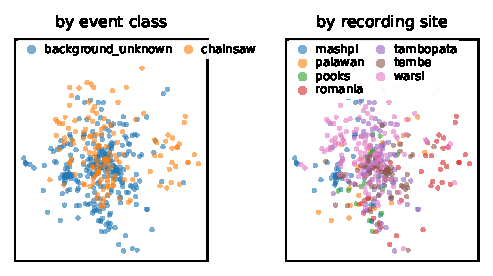
\includegraphics[width=\columnwidth]{figures/pca_cnn_threat_cnn_kaggle_augmented_v1.pdf}
\caption{PCA of the supervised-CNN embedding of held-out forest clips, colored by
event class (left) and by recording site (right). Structure tracks site at least
as strongly as class.}
\label{fig:pca}
\end{figure}

\paragraph{Takeaway.} Closed-set classifiers fail under site-level shift not
because they cannot discriminate threats, but because (i) their operating point,
calibrated on the source domain, does not transfer, and (ii) their representation
encodes site-specific structure. This motivates a detector whose decision
boundary is defined by the \emph{deployment site's own} background and whose
attribution is decoupled from a frozen, general-purpose representation, the
design of Section~\ref{sec:method}.

\section{Method}
\label{sec:method}

Let $\phi: \mathcal{X} \to \mathbb{R}^d$ be a fixed embedding of an audio clip.
We deliberately \emph{freeze} $\phi$: the detector never backpropagates into it,
so a new class or a new site never triggers retraining. All learning happens in
two lightweight, closed-form stages over embeddings.

\subsection{Stage 1: Background density and flagging}

Given embeddings $\{\phi(x_i)\}$ of unlabeled forest-at-rest clips, we fit a
Gaussian with a shrunk covariance for a well-conditioned inverse
\citep{ledoit2004shrinkage}:
\begin{equation}
\hat\Sigma = (1-\alpha)\, S + \alpha\, \mathrm{diag}(S) + \epsilon I,
\end{equation}
where $S$ is the sample covariance and $\alpha$ the shrinkage. A clip's raw
anomaly is its Mahalanobis distance \citep{lee2018mahalanobis}
$r(x) = \sqrt{(\phi(x)-\hat\mu)^\top \hat\Sigma^{-1} (\phi(x)-\hat\mu)}$.
Raw distances are not comparable across sites, so we map them through the
\emph{empirical background CDF}: the anomaly score $s(x)\in[0,1]$ is the
quantile of $r(x)$ among training-background distances, so $s = 0.99$ means
``more unusual than 99\% of this forest's background.''

\paragraph{FP-budget calibration.} We flag when $s(x) \ge \tau$. Rather than a
fixed $\tau$, we pick the smallest threshold whose background false-positive
rate on a held-out background split is at most a budget $\beta$ (we use
$\beta = 0.10$, the platform's promotion gate). This maximizes recall subject to
the ranger-attention budget and is the only quantity a site operator must set.
Crucially, Stage~1 needs \emph{no labeled positives}.

\subsection{Stage 2: Open-set attribution}

For each known class $c$ with verified positives, we store an
$L_2$-normalized mean prototype $p_c = \widehat{\mathrm{mean}}_i\, \widehat{\phi(x_i)}$.
For a flagged clip we compute cosine similarities $\sigma_c = p_c^\top \hat\phi(x)$
and split the probability mass into a known part and an honest unknown part.
Letting $\sigma^\star = \max_c \sigma_c$ and a similarity floor $\theta$, the
known mass is
\begin{equation}
m = \mathrm{clip}\!\left(\frac{\sigma^\star - \theta}{1 - \theta},\, 0,\, 1\right),
\end{equation}
distributed over classes by a temperature-softmax of $\{\sigma_c\}$, with the
remaining $1-m$ assigned to \emph{unknown}. With zero prototypes, $m = 0$ and
every anomaly is honestly unknown, and flagging is unaffected. As verified
positives arrive for a class, its prototype sharpens and its mass grows,
\emph{monotonically and without retraining}, which is exactly the incremental
behavior a ranger-in-the-loop deployment needs.

\subsection{Embedding choice}

$\phi$ is pluggable. We compare a site-trained CNN's pre-classifier feature
($64$-d) against two frozen general-purpose encoders: AudioSet-pretrained CNN14
($2048$-d) and BirdNET V2.4 ($1024$-d), a bioacoustics encoder trained for bird
vocalization. All three are evaluated under identical background-density and
prototype machinery. Because Stage~1 and Stage~2 are closed-form over
embeddings, swapping $\phi$ is the only change required to test a new
representation, which is what lets us attribute cross-site performance to the
representation rather than the detector.

\section{Experiments}
\label{sec:experiments}

\paragraph{Data and protocol.} We use RFCx rainforest soundscapes
\citep{rfcx_frugalai} with chainsaw and background labels from four sites carrying enough of both for a per-site
estimate: warsi ($412$ chainsaw / $198$ background test clips), tambopata
($41/72$), romania ($30/15$), pooks ($10/12$). Every experiment is
\emph{leave-one-site-out}: all clips from the target site are reserved for test,
everything is fit on the remaining sites, and the decision threshold is
calibrated on a training-site background validation split at a background
false-positive budget of $0.10$. A recording-level audit confirms zero clips from
the held-out site in train or validation and zero shared source recordings across
splits, so no result below is contaminated by clip-window leakage.

\paragraph{Metrics.} \emph{Flagged recall} (positives scoring above threshold),
\emph{attributed recall} (flagged \emph{and} the predicted kind is correct),
\emph{background FP}, and threshold-free AUC of the score separating chainsaw
from background. For the supervised probe we additionally report
\emph{event-level recall}: clips are grouped back into source recordings and an
event counts as detected if any of its clips fires, since a chainsaw runs
continuously and the operational unit is the event, not the $3$-second clip.

\paragraph{Implementation and reproducibility.} The detector and evaluation math
are NumPy and unit-tested ($123$ tests); audio inference uses PyTorch~2.7 with
\texttt{panns\_inference} (AudioSet CNN14, $2048$-d) and \texttt{birdnetlib}
(BirdNET V2.4, $1024$-d) on CPU/Apple-Silicon under macOS. Randomized results fix
seeds and every interval is a $1000\times$ bootstrap. All numbers below were
regenerated from scratch for this submission; code, fitted artifacts, manifests,
and the exact commands are released. The evaluation audio is public and released
under CC BY-NC 4.0; the closed-set lineage additionally trains on public forest
and urban corpora \citep{bandara2023fsc22,gemmeke2017audioset}.

\subsection{From diagnosis to a deployable operating point}

Section~\ref{sec:diagnosis} established that closed-set classifiers fail across
sites through operating-point transfer and site encoding. Table~\ref{tab:headline}
compares, on the primary held-out site, the strongest closed-set baseline against
the open-set detector under two embeddings. The closed-set model is a CNN trained
on rainforest audio \emph{with tambopata held out}, the most favorable closed-set
setting: $0.976$ chainsaw recall at raw argmax, but with half of all background
flagged as a threat; calibrated to a deployable false-positive rate, recall
collapses to $0.195$. Re-using that same CNN as the open-set \emph{embedding}
inherits the site bias, giving an anomaly-score AUC of $0.319$, below chance, and
consistent with the representation analysis in Section~\ref{sec:diagnosis}.
Swapping in a frozen AudioSet encoder is what recovers a usable operating point.

\begin{table}[t]
\centering
\caption{Held-out-site (tambopata) chainsaw detection, threshold calibrated to
background FP $\le 0.10$ on training-site validation. All rows are our own
re-run under one protocol. ``Score AUC'' is threshold-free separability
\emph{before} any labels are used.}
\label{tab:headline}
\small
\begin{tabular}{lrrr}
\toprule
Method & Recall & Bg FP & Score AUC \\
\midrule
Closed-set CNN (raw argmax)       & 0.976 & 0.500 & --- \\
Closed-set CNN (calibrated)       & 0.195 & 0.000 & --- \\
Open-set, site-trained CNN        & 0.049 & 0.028 & 0.319 \\
Open-set, AudioSet CNN14          & \textbf{0.317} & 0.056 & \textbf{0.713} \\
\bottomrule
\end{tabular}
\end{table}

\begin{table}[t]
\centering
\caption{Leave-one-site-out folds, open-set (background-only) detector.
The AudioSet embedding lifts separability above chance at every site where the
site-trained CNN is at or below it, but the validation-calibrated threshold does
not always hold the FP budget on an unseen site. pooks has only $10$ held-out
chainsaw clips and should be read as indicative.}
\label{tab:folds}
\small\setlength{\tabcolsep}{4pt}
\begin{tabular}{lrrrrr}
\toprule
& & \multicolumn{2}{c}{site-trained CNN} & \multicolumn{2}{c}{AudioSet CNN14} \\
\cmidrule(lr){3-4}\cmidrule(lr){5-6}
Site & $n_{\text{ch}}$ & Recall & AUC & Recall & AUC \\
\midrule
tambopata & 41  & 0.049 & 0.319 & 0.317 & \textbf{0.713} \\
warsi     & 412 & 0.250 & 0.481 & 0.367 & 0.619 \\
romania   & 30  & 0.167 & 0.564 & 0.267 & 0.559 \\
pooks     & 10  & 0.000 & 0.146 & 0.000 & 0.546 \\
\bottomrule
\end{tabular}
\end{table}

\subsection{The representation, not the head, governs transfer}

Because the open-set machinery is identical across embeddings, the comparison
isolates the effect of the frozen encoder $\phi$. The site-trained CNN inherits
the domain bias that sinks the closed-set model (AUC $0.15$--$0.56$, at or below
chance), whereas the frozen AudioSet encoder is above chance at every held-out
site ($0.55$--$0.71$; Table~\ref{tab:folds}). On the primary site it reaches
$0.317$ flagged recall at $0.056$ background FP, exceeding the closed-set
calibrated recall of $0.195$ while using \emph{zero} labeled positives to decide
what is anomalous.

Two caveats temper this. Absolute recall is modest ($0.27$--$0.37$ where the FP
budget is met): faint, distant chainsaws under an unseen chorus remain hard.
And the threshold calibrated on training-site background does not always hold the
budget on an unseen site (warsi $0.20$, romania $0.13$), a cross-site
\emph{calibration} gap distinct from the separability the embedding provides.

\subsection{What label-free operation costs}
\label{sec:cost}

To separate what is lost by using no labels from what is lost to site shift, we
fit a supervised probe (logistic regression) on the \emph{same} frozen embeddings
using the training-site chainsaw labels a real deployment eventually accumulates,
under the identical leave-one-site-out protocol and FP budget
(Table~\ref{tab:probe}, Figure~\ref{fig:transfer}). This is the label-rich upper
bound for a given representation.

\begin{table}[t]
\centering
\caption{Supervised leave-one-site-out probe over frozen embeddings, at the same
$0.10$ background-FP budget. AUROC is threshold-free, event recall groups clips
into source recordings. Rows are $n$-weighted means over the four folds; per-site
AUROC $95\%$ CIs are bootstrap. The choice of representation moves transfer far
more than the choice of head.}
\label{tab:probe}
\small
\begin{tabular}{lrrr}
\toprule
Frozen embedding & AUROC & Clip recall & Event recall \\
\midrule
site-trained CNN & 0.648 & 0.369 & 0.370 \\
AudioSet CNN14   & 0.783 & \textbf{0.594} & \textbf{0.595} \\
BirdNET V2.4     & \textbf{0.786} & 0.527 & 0.531 \\
\bottomrule
\end{tabular}
\end{table}

\begin{figure*}[t]
\centering
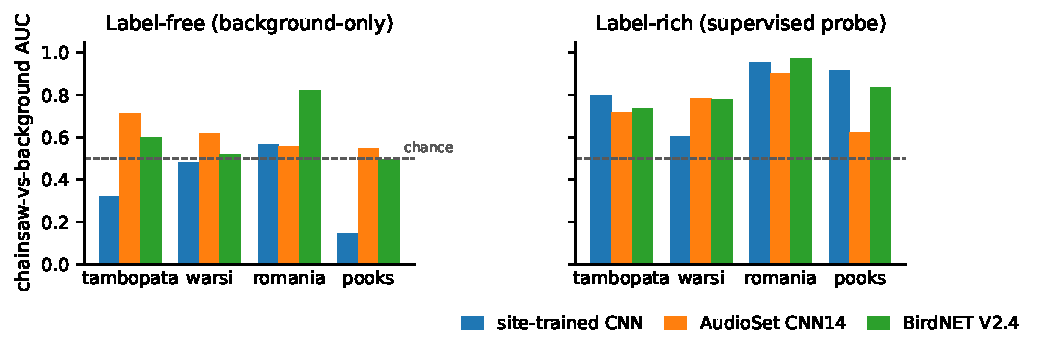
\includegraphics[width=\textwidth]{figures/transfer.pdf}
\caption{Per-site chainsaw-vs-background AUC, label-free (left) and label-rich
(right), for the three frozen embeddings. Dashed line is chance. General-purpose
audio representations transfer; the site-trained one does not.}
\label{fig:transfer}
\end{figure*}

Three findings follow. First, the general-purpose encoders are far better
substrates than the site-trained CNN: weighted AUROC $0.783$ (AudioSet) and
$0.786$ (BirdNET) against $0.648$, and on romania BirdNET reaches AUROC $0.973$
with $0.966$ event recall at $0.067$ FP, an operationally useful detector.
Second, the two general encoders are near-tied on AUROC despite very different
pretraining (AudioSet tagging versus bird vocalization), which points to generic
acoustic generality rather than any threat-specific prior as the active
ingredient. Third, comparing Table~\ref{tab:probe} with Table~\ref{tab:folds}
prices label-free operation: with labels, the AudioSet representation supports
$0.594$ event recall; without them, background-only flagging on the same
representation delivers $0.317$ on the primary site. Labels roughly double
recall, but the label-free detector is the one that can run on day one.

\subsection{Ranking can be strong while calibration fails}

BirdNET makes the paper's central distinction unusually sharp. As a supervised
probe it is the best embedding we tested (weighted AUROC $0.786$). Yet under
the label-free detector it flags \emph{nothing} at every site (recall $0.000$),
despite threshold-free AUC up to $0.821$ on romania. The score ranks chainsaws
above background; the background-density threshold calibrated on training sites
simply lands in the wrong place on an unseen one. This is the same
operating-point failure we diagnosed in the closed-set classifier
(Section~\ref{sec:diagnosis}), reappearing in a fully unsupervised detector, and
it is why we report recall at a fixed FP budget rather than AUC alone: an
embedding can be excellent and still be undeployable if its operating point does
not transfer.

\subsection{Attribution lights up with a handful of labels}

Figure~\ref{fig:kcurve} plots attributed recall against the number of verified
positives per class $k \in \{0,1,5,10,25\}$, with flagging held fixed. At $k=0$
every anomaly is honestly unknown by construction ($0.000$ attributed recall); on
tambopata attribution rises to $0.112$ at $k=5$ and $0.180$ at $k=25$. Flagging
is identical across all $k$ by construction, so ranger confirmations only move
mass from \emph{unknown} onto the named class, which is the day-one-useful,
self-improving behavior a human-in-the-loop deployment needs.

\begin{figure}[t]
\centering
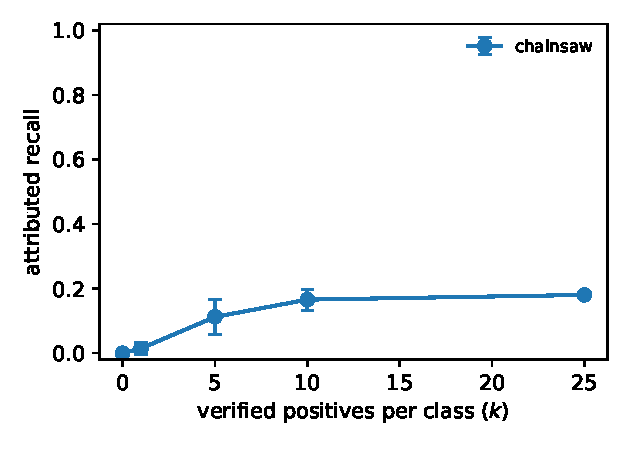
\includegraphics[width=0.85\columnwidth]{figures/kcurve.pdf}
\caption{Attributed recall vs.\ verified positives per class (tambopata
held-out, AudioSet embedding; mean $\pm$ std over seeds). Flagging is independent
of $k$; only attribution depends on it.}
\label{fig:kcurve}
\end{figure}

\subsection{Honest unknowns}

To test abstention we remove chainsaw's prototype entirely and re-score the
held-out site's chainsaw clips. A well-behaved open-set detector should still
\emph{flag} them, since they remain acoustically unusual, while assigning their
likelihood mass to \emph{unknown} rather than misattributing it to a remaining
class. This is what we observe: flagging is unchanged and $100\%$ of flagged
clips are predicted \emph{unknown} with mean unknown mass $1.0$. The detector
never invents a label for a class it was never shown.

\subsection{Limitations}

Our evidence is one threat class (chainsaw) across four rainforest sites, and two
folds are small ($n=30$ and $n=10$), so per-site numbers carry wide intervals and
we weight by $n$ when aggregating. Absolute label-free recall remains modest, and
the calibration gap means an operator should expect to spend a small amount of
destination-site background to place the threshold. We evaluate on recorded
clips, not a live deployment; a field study with in-situ positives is the
necessary next step and is underway.

\section{Deployment: The Ranger-in-the-Loop Flywheel}
\label{sec:deployment}

The detector ships inside an open-source forest-monitoring platform that we
release with this paper (name withheld for anonymous review).
A field sensor uploads a clip; the API scores it with the fitted detector and,
when $s(x)\ge\tau$, creates an anomaly alert carrying the anomaly score, the
predicted kind, and the full likelihood vector including \emph{unknown}. The
dashboard renders the ranked breakdown (e.g.\ ``likely chainsaw 71\% $\cdot$
vehicle 12\% $\cdot$ unknown 17\%'') so a ranger sees not just \emph{that}
something is unusual but the current best guess and its uncertainty.

\paragraph{Closing the loop without retraining.} Ranger confirmations in the
clip-review UI are exported as a positives manifest and folded back into the
prototype set. Because attribution is closed-form over a frozen embedding, this
is a seconds-long refit, not a training run: the very labels the deployment
generates are the labels that light up its classes. This is the operational
realization of the $k$-curve in Section~\ref{sec:experiments}: each
confirmation moves the system rightward along it.

\paragraph{Why background-first fits social-impact constraints.} Under-resourced
conservation teams cannot commission labeled threat corpora for every reserve,
but every site can record its own background on day one. Anchoring the detector
to background makes the expensive resource (labeled positives) optional and
incremental, and makes the tunable knob a single interpretable
quantity, the background false-positive budget that bounds wasted ranger
patrols. The honest \emph{unknown} option means a novel threat (a new machine, a
new vehicle) is surfaced rather than silently misfiled, which is the failure
mode a fixed taxonomy cannot avoid.

\paragraph{Reproducibility.} The detector math is a small, dependency-light
module unit-tested without the audio stack; the fit and evaluation are single
commands over public manifests; and fitted artifacts, the evaluation protocol,
and the platform are released open-source. We complete the AAAI reproducibility
checklist and document dataset licenses for redistribution.

\section{Conclusion}

Closed-set acoustic threat classifiers do not survive a change of forest: strong
in-domain validation hides a cross-site collapse once a deployable
false-positive budget is enforced, and the collapse is one of operating-point
transfer rather than discrimination, driven by a representation that encodes
recording site more strongly than event class. We reframed the task as
background-first and open-set, flagging deviation from a site's own soundscape,
attributing with incrementally built prototypes, and abstaining honestly. The
resulting detector ships with zero labeled threats and improves as rangers
confirm alerts, without retraining.

Across four held-out sites the choice of frozen representation, not the detector
head, governed transfer, and a supervised probe on the same embeddings priced
what label-free operation costs: labels roughly double recall, but only the
label-free detector can run on day one. BirdNET sharpened the central lesson by
being the strongest probe substrate while flagging nothing under a transferred
threshold, a reminder that ranking quality and deployability are different
properties and that false-positive control is what binds.

Beyond forests, the same recipe fits any monitoring setting where normal is easy
to record, anomalies are rare and open-ended, and expert attention is the
limiting resource. Limitations remain: one threat class, four sites, two of them
small, modest absolute recall, and a calibration gap that a little
destination-site background should close. Field validation on in-situ positives
is the necessary next step and is underway.


\bibliography{references}

% Reproducibility checklist: compiles standalone (`pdflatex ReproducibilityChecklist`)
% for separate submission, or append it to this paper by uncommenting the two
% lines below. Keep it out of the 7+2 main-content page count unless the track
% requires it inline.
% \makeatletter\def\isChecklistMainFile{}\makeatother
% \input{ReproducibilityChecklist.tex}

\end{document}
